\chapter{Úvod}
    Svět her je pro umělou inteligenci jedno z velkých témat. Hra by nemohla být zábavná, kdyby nepřítel nebyl dostatečně chytrý. Umělá inteligence silného oponenta ve složité hře představuje disciplínu stále otevřenou novým technikám, metodám a možnostem. Výpočetní náročnost takových her staví velkou překážku k vytvoření \textit{ideální} umělé inteligence například pro hru Go. Ačkoliv se již v minulosti podařilo překonat člověka například v hře Šachy, stále je to malý krůček pro tak velký svět zajímavých rozhodovacích problémů jakým je i Ms. Pacman. Ms. Pacman patří k těmto složitým úlohám nejen rozměrností stavů, jež ve hře můžou nastat, ale především náhodností chování svých oponentů, duchů. Nelze tedy přesně stanovit, jak se daný duch bude v danou situaci chovat, lze jen jaksi předpokládat, tudíž je těžší jednoznačne stanovit, jak se má umělá inteligence Ms. Pacman chovat.

Cílem této práce je navrhnout a implementovat dostatečně chytrou umělou inteligenci Ms. Pacman, a to v podobě inteligentního agenta, který bude co nejlépe reagovat na své aktuální prostředí a to tak, aby jeho inteligence překonala problematiku náhodnosti a vypočetní náročnosti této hry. Kvalita agenta bude srovnána s již známými metodami řešení podobných problémů. Práce je rozdělena na dvě části, z nichž první se zaměřuje na teoretický základ, popis a klasifikaci samotného problému. Praktická část popisuje návrh a implementaci zmíněných algoritmů.
1
\chapter{Metody hraní her}
Tato kapitola si klade za cíl seznámit čtenáře s metodami hraní her. Hry úzce souvisí s metodami řešení úloh, zahrnují tedy snahu dostat se z počátečního stavu do cílového, např. za použití posloupnosti nějakých pravidel. 

\section{Základní pojmy}

\subsection*{Stavový prostor}
Stavový prostor \cite{AI1} je množina všech stavů, které mohou ve hře nastat. Stavový prostor lze reprezentovat jako orientovaný graf, jehož \textit{uzly} představují jednotlivé pozice ve hře (stavy) a orientované hrany přechody mezi jednotlivými stavy, tedy přípustné tahy ve hře. První uzel se nazývá \textit{kořen}, koncové uzly, \textit{listy}, pak reprezentují koncové pozice ve hře (cíly, stavy). Na obrázku \ref{img:stavp} lze vidět ukázku omezeného (zjednodušeného) stavového prostoru hry Pacman. Velikost takto velmi omezeného stavového prostoru musí vzít v potaz: rozměry 2D hracího pole, 4 možné směry pohybu Pacmana a fakt, zda 8 kuliček jídla už (ne)bylo snězeno, tedy:  $3 \times 3 \times 2^{8} \times 4 = 9 216$ (!) stavů a to nebyl brán v potaz ani jediný nepřítel, natožpak reálná velikost hracího pole desky.
\newline
K dosažení každého uzlu je potřeba vydat nějaké úsilí, \textbf{cenu} \cite{AI1}, která tedy udává nezáporné ohodonocení hrany z jednoho uzlu k druhému. \textbf{Hloubka uzlu} \cite{AI1} udává počet hran na cestě od počátečního uzlu k danému uzlu. Kořen má hloubku 0, jeho následníci mají hloubku 1 atp.


\begin{figure}[h]
\begin{center}
	\scalebox{0.7}{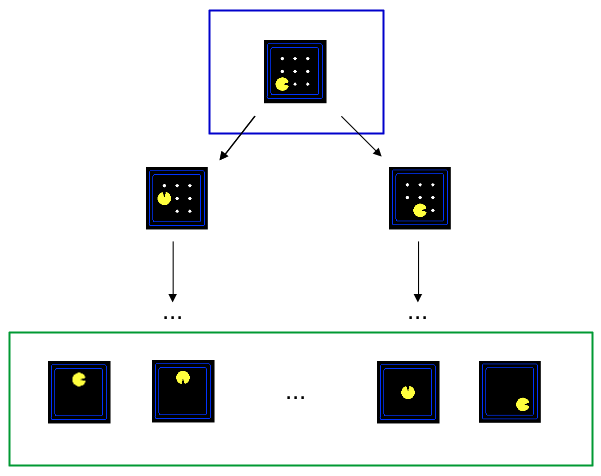
\includegraphics{img/statespace.png}}
	\caption{Ukázka stavového prostoru pro hru Pacman. Každý pohyb Pacmana znamená nový stav hry, tedy uzel. Modrý obdélník ohraničuje počáteční stav, kořen, a zelený obdelník ohraničuje možné koncové stavy, listy.}
	\label{img:stavp}
\end{center}
\end{figure}

\subsection*{Optimální versus nejlepší řešení}
Další důležitou součástí metod řešení úloh je \textbf{hodnotící funkce} (\textit{successor function}) \cite{AI1}. Jedná se o funkci vyhodnocující celkovou cenu od jednoho uzlu k druhému, např. součet ceny a \textit{heuristické funkce}.
\textbf{Heuristická funkce} \cite{berkeley} je založena na empirických znalostech (až odhadech) o hře, používaná při prohledávání stavového prostoru. Může to být například vzdálenost Ms. Pacman vůči svému cíli. Podle jejího využití dělíme algoritmy na \textbf{informované} a \textbf{neinformované} \cite{AI1}.
Proč ale používáme heuristiku místo jistějšího systematického prohledávání stavového prostoru, které by mělo definovat vlastně \textit{nejlepší} řešení? Je to především kvůli velké vypočetní náročnosti toho způsobu prohledávání a vyhodnocování celého stavového prostoru, který u složitějších problémů nabývá příliš velkých rozměrů, aby se vše stihlo provést, např. v reálném čase při hraní hry. Pokud je heuristika \textit{optimální}, zaručuje zvýšení efektivity a rychlosti.
\newpage
\subsection*{Vlastnosti algoritmů}
Rozlišujeme několik následujících vlastností algoritmů\cite{AI1}:
\begin{itemize}
\item \textbf{Úplnost} – Pokud existuje řešení, je garantováno, že ho algoritmus vrátí?
\item \textbf{Optimálnost} – Je garantováno nalezení nejlepší řešení, tedy řešení s nejmenší cenou?
\item \textbf{Časová složitost} – Kolik uzlů je nutno expandovat? Kolik to zabere času v nejhorším/nejlepším případě/průměrně?
\item \textbf{Prostorová složitost} – Kolik dat je nutno si uchovávat v paměti v nejhorším/nejlepším případě/průměrně?
\end{itemize}

\section{Hry}
\textbf{Hra} (také se označuje jako \textit{adversarial search}) je z matematického hlediska rozhodovací problém, ve kterém figurují 2 a více účastníků, hráčů \cite{AI1}. Hráči se snaží chovat racionálně, viz sekce \ref{sec:racionalita}.
\newline
\textbf{Složité hry} \cite{AI1} jsou hry s tak velkým úplným stavovým prostorem, že by jeho neinformované prohledávání nebylo možné výpočetně zvládnout. Například šachy, Go, Ms. Pacman. V takových případech je potřeba omezit strom stavového prostoru pomocí hloubky, tedy maximálního počtu kroků dopředu oproti aktuálnímu stavu, a použít \textit{statickou hodnotící funkci}, která určuje \textit{pravděpodobnost} dosažení cíle z aktuálního stavu. Následující metody hraní her potřebují mít úplnou informaci o stavovém prostoru hry.
\subsection{Minimax}
Metoda \cite{AI1} prohledávání do hloubky s omezením hloubky prohledávání. Hodnotící funkce nám udává určitou \textit{hodnotu} listů $V(s)$, tedy nejlepší výsledek/užitek, kterého lze dosáhnout z aktuálního stavu.
Následně se úrovni hráče při procházení stavového prostoru vybírá \textbf{maximum hodnoty:} $V(s) = \max \: V(s^\prime)$, kde $s^\prime \in naslednici(s)$. 
\newline
Na úrovni protihráče \textbf{minimum hodnoty:} $V(s^\prime) = \min \: V(s)$, kde $s \in naslednici(s^\prime)$. Hráči se takto rekurzivně střídají od listů až po finální výpočtení hodnoty kořene.

\subsection{AlfaBeta řezy}
Metoda pro zmenšení stavového prostoru \cite{AI1}, odříznutím nadbytečných větví. Využívá dvou \textit{mezí}:
\begin{itemize}
\item \boldmath$\alpha$ reprezentující dolní mez ohodnocení uzlu, tedy tah hráče
\item \boldmath$\beta$ reprezentující horní mez ohodnocení uzlu, tedy tah protihráče
\end{itemize}
Algoritmus si pamatuje hodnoty svých mezí, a postupně je aktualizuje porovnáváním meze s následníky uzlu aktuální úrovně a to podle toho, na které úrovni se nachází: ($max$ - aktualizuji $\alpha$ na největší hodnotu následníků, $min$ - aktualizuji $\beta$ na nejmenší hodnotu následníků). Porovnávání probíhá dokud $\alpha < \beta$, takto se vynechají nadbytečné větve, jejichž procházení již nezmění výslednou cestu. Konečná hodnota kořene je stejná jako u Minimaxu, a pokud by se uzly správně seřadily, výrazně se tím změní vypočetní náročnost algoritmu. 
\subsection{Expectimax}
Expectimax \cite{mas} je jednou z možností jak řešit \textbf{hry s neurčitostí} jako je i Ms. Pacman. Hry s neurčitostí také zahrnují střídání hráčů a mají také úplnou informaci o stavu hry, avšak navíc využívají při získání těchto informací \textit{pravděpodobnosti}, které popisují náhodný charakter stavů ve hře. Příkladem jsou hry, kde figuruje házení kostkou nebo např. řízení libovolného robota v reálném světě, kdy se může náhodně pokazit nějaká jeho součástka. Expectimax obohacuje každý tah hráče (jako Minimax) o náhodnost. \textbf{Hodnoty stavů} nyní navíc reflektují průměrnou pravděpodobnost stavů: \newline \newline
$V_{\min}(s) = \sum_{i=0} p_i * \min \: V(s^\prime)$, kde
\newline $s^\prime \in naslednici(s)$ a $p_i$ je pravděpodobnost daného stavu $i$-té úrovně.
\newline
\newline
$V_{\max}(s^\prime) = \sum_{i=0} p_i * \max \: V(s^\prime)$, kde 
\newline
$s^\prime \in naslednici(s)$ a $p_i$ je pravděpodobnost daného stavu $i$-té úrovně.
\newline
\newline
Tyto rovnice udávají tzv. \textbf{očekávaný užitek} (\textit{expected utility}) dané úrovně \cite{mas}. Na obrázku \ref{img:expectimax} lze vidět použití algoritmu.

\begin{figure}[h]
\begin{center}
	\scalebox{0.35}{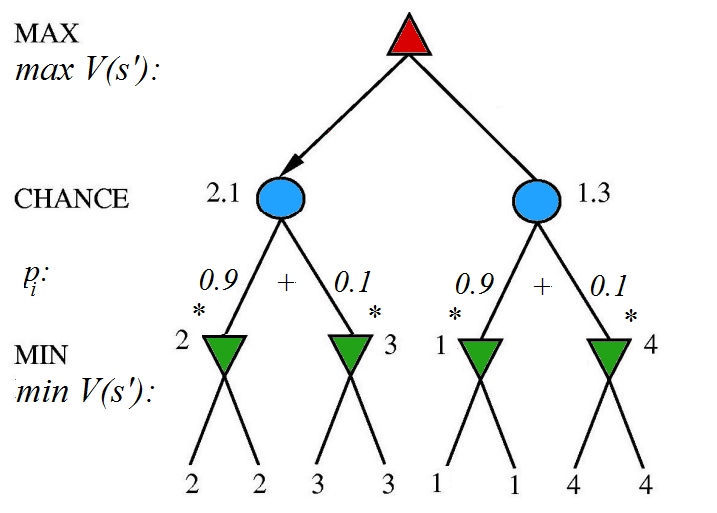
\includegraphics{img/expectimax.png}}
	\caption{Na obrázku lze vidět ukázku vyhodnocování náhodných uzlů a výslednou cestu \boldmath$A_1$, kterou si algoritmus posléze zvolí.}
	\label{img:expectimax}
\end{center}
\end{figure}

\chapter{Učící agent}
Tato kapitola se zaměřuje na teoretický podklad hlavního cíle práce, inteligentní formu reaktivního agenta \cite{AI3}.
\section{Reaktivní agent}
Reaktivní agent \cite{AI3} se dá představit jako autonomní bot, který reaguje na své aktuální okolní prostředí. Nebere tedy v potaz následky svého konání. Matematicky lze zapsat \textit{šesticí} \cite{AI3} jako: $(S,T,A, vjem, ukon, akce)$, kde:
\begin{itemize}
\item $S$ je množina okolních stavů agenta,
\item $T, T\subseteq S$ je okolí, které může agent vnímat,
\item $vjem: S \to T$ je agentem právě vnímaný stav okolí ($s \in S$)
\item $A$ je množina možných úkonů, jež může agent v daný stav vykonat,
\item $ukon: A \times A \to S$ je vykonaný úkon, jež má za následek změnu prostředí $S$
\item $akce: T \to A$ je vybraná akce na základě $vjemu$.
\end{itemize}
Agent představuje účastníka hry (hráče).

\section{Racionalita}
\label{sec:racionalita}
Každý hráč má nějaký cíl a k němu vedoucí strategii. Strategie se skládá z hráčových akcí a voleb, které pro hráče vedou k vlastnímu užitku (\textit{utility}), potažmo výhře. Hráč se potýká s různými stavy ve hře a snaží se z nich vytěžit co nejvíce na základě svých preferencí \cite{berkeley}. Pokud tyto hráčovy preference dodržují axiomy dle \cite{mas}, zaručují tak hráčův cíl, maximalizaci očekávané hodnoty \textit{užitkové funkce}:
\begin{displaymath} 
U([p_1,S_1;\dots;p_n,S_n]) = \sum_{i}p_iU(S_i)p
\end{displaymath}
Pro umělou inteligenci hráče je též důležité explicitně stanovit určitá pravidla, ze kterých má hráč vybírat užitek. Předpoklad racionality je hlavní rozdíl teorie her a teorie rozhodování.

\section{Markovský rozhodovací proces}
Agent se bude pohybovat ve \textit{stochastickém} (náhodném) prostředí, je tedy vhodné si definovat Markovský rozhodovací proces \cite{RLAprox}, dále \textbf{MDP} (\textit{Markov decision process}), který řeší takovéto nedeterministické problémy prohledávání, jedná se o čtveřici:
$(S,A,T,R)$, kde:
\begin{itemize}
\item $s, s \in S$ je množina stavů, která zahrnuje počáteční a koncový stav
\item $a, a \in A$ je množina akcí
\item $T(s,a,s^\prime)$ je \textbf{přechodová funkce} (\textit{transition function}), nebo též \textit{model}, tedy pravděpodobnost přechodu ze stavu $s$ do $s^\prime$ ($P(s^\prime| s, a) $)
\item $R(s,a,s^\prime)$ je  \textbf{odměnová funkce} (\textit{reward function}), s ní souvisí exponenciální snižování hodnot odměn koeficientem $\gamma$ (\textit{discount})
\end{itemize}
Důležitý rozdíl proti předchozím metodám hraní her je fakt, že výsledná hodnota aktuálního stavu závisí pouze na aktuálním stavu a jeho akci, ne na jeho historii.
Další významný rozdíl je ten, že předchozí metody se snažily o nalezení optimálního plánu nebo sekvence akcí z počátečního stavu až do cíle. MDP hledá \textbf{optimální strategii} (\textit{policy}) -ZDROJ-:
\begin{displaymath}
\pi^*: S \to A
\end{displaymath}
$\pi$ mapuje akci na každý stav a pokud se akce provede, maximalizuje očekávaný užitek.

\textbf{Užitek} -ZDROJ- je definován jako suma koeficientem $\gamma$ snížených odměn tak, aby MDP měl větší šanci skončit (pro agenta je lepší vzít blízkou odměnu co nejdříve, tudíž optimálněji sbírá odměny).

\textbf{Hodnota} -ZDROJ-definuje \textbf{optimální očekávaný užitek} (akumulovaný průměr očekávaných výsledků) ze stavu (pro uzly max/min)

\subsection{Value iteration a Policy iteration}
Příkladem přepočtu hodnot je metoda \textbf{Value iteration} \cite{RLAprox}:
\begin{enumerate}
\item začni od úrovně s hodnotou $V_{0} = 0$
\item plň vektor optimálních hodnot $V_{k}(s)$ novými hodnotami vykonáním Expectimaxu pro aktuální úroveň pomocí rovnice:\footnote{$\gamma V_k(s^\prime)$ je hodnota budoucí odměny}
\begin{displaymath}
V_{k+1}(s) \leftarrow \max_a \sum_{s^\prime}T(s,a,s^\prime) \left[R(s,a,s^\prime)+\gamma V_k(s^\prime) \right]
\end{displaymath}
\item opakuj předchozí krok dokud vektor $V_k$ nekonverguje (konvergenci především zapřičiňuje $\gamma$, což zaručuje optimálnost metody): $\left|V_{k+1}(s)-V_k(s) \right| < presnost$.
\end{enumerate}
Velký rozdíl oproti Expectimaxu je ten, že se nemusí provádět neustálá \textit{rekurze} výpočtu očekávaného užitku, protože je už vypočten ve vektoru hodnot $V_k(s^\prime)$. Stále se však metoda potýká s vysokou prostorovou složitostí. Alternativou jsou proto metody \textbf{Policy iteration} \cite{RLAprox}, které se snaží o přímé nalezení optimální strategie raději než zdlouhavé výpočty hodnot. O těchto metodách se v souvislosti se strojovým učením zmiňuje další kapitola \ref{sec:rl}.

\subsection{Q-hodnota}
Posledním důležitým pojmem je Q-hodnota -ZDROJ-, která definuje optimální očekávaný užitek v budoucnosti z uzlu náhodnosti, tzv. \textit{q-stavu}, příklad na obrázku \ref{img:qvals}.

Pro získávání optimálních $V$-hodnot a $Q$-honot  v MDP tedy platí následující rovnice:\footnote{hvězdička $^{*}$ značí optimální hodnotu}, \footnote{rovnice přímo vychází z Bellmanových rovnic \cite{mas}}
\begin{displaymath}
V^*(s) = \max_a Q^*(s) (s,a,s^\prime)
\end{displaymath}
\begin{displaymath}
Q^*(s) = \sum_{s^\prime}T(s,a,s^\prime) \left[R(s,a,s^\prime)+\gamma V_k(s^\prime) \right]
\end{displaymath}

Na obrázku \ref{img:policy} lze vidět optimální strategii a vypočtené hodnoty pro daný \textit{grid-world} problém.

\begin{figure}[!htbp]
\begin{center}
	\scalebox{0.55}{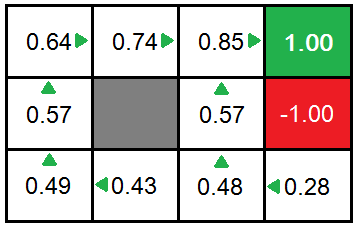
\includegraphics{img/policy.png}}
	\caption{Problém představuje pole o velikosti 12 polí (z nichž šedé je nedosažitelné), 4 směry možnosti chůze a dva koncové stavy s odměnami ohodnocenými -1 a 1. Již po 5 iteracích je vidět optimální strategie, reprezentovaná šipkou směru (agent začíná v levém spodním rohu), vypočtena pomocí hodnoty $V_{5}$ každého pole.}
	\label{img:policy}
\end{center}
\end{figure}

\begin{figure}[!htbp]
\begin{center}
	\scalebox{0.6}{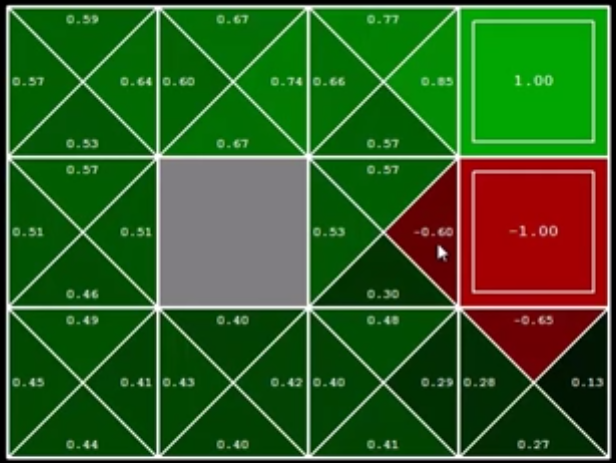
\includegraphics{img/qvals.png}}
	\caption{Ukázka počátečních Q-hodnot pro předešlý grid-world problém (po 5. iteraci). Q-hodnoty se počítají pro všechny možné akce z daného stavu, proto jsou pro jedno políčko na hracím plánu 4 pro každý směr, kam může agent jít.}
	\label{img:qvals}
\end{center}
\end{figure}
MDP lze též reprezentovat prohledávacím stromem, viz obrázek \ref{img:mdptree}, který se velmi podobá Expectimaxu avšak jak již bylo řečeno není potřeba rekurze.

\begin{figure}[!htbp]
\begin{center}
	\scalebox{0.5}{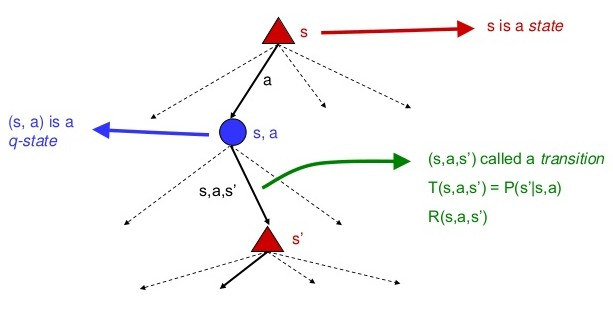
\includegraphics{img/mdptree.jpg}}
	\caption{Na obrázku lze vidět analogii MDP k Expectimaxu \cite{RLIntro}.}
	\label{img:mdptree}
\end{center}
\end{figure}
\newpage
\section{Strojové učení}
\label{sec:rl}
Další důležitou vlastností agenta bude schopnost \textit{učit se} \cite{RLIntro}. Agent se učí na pozorovaných výsledcích svých akcí, tzv. \textbf{vzorky} $(s,a,s^\prime,r)$, kde $r$ je odměna nového stavu. Stále se jedná o MDP, avšak největší rozdíl zde nastává v tom, že \textbf{neznáme} odměnovou funkci \boldmath$R$, ani přechodovou funkci \boldmath$T$. Agent (viz obrázek \ref{img:learningagent})se tedy musí metodou \textit{pokus-omyl} NAUČIT tyto hodnoty modelu.

\begin{figure}[!htbp]
\begin{center}
	\scalebox{0.25}{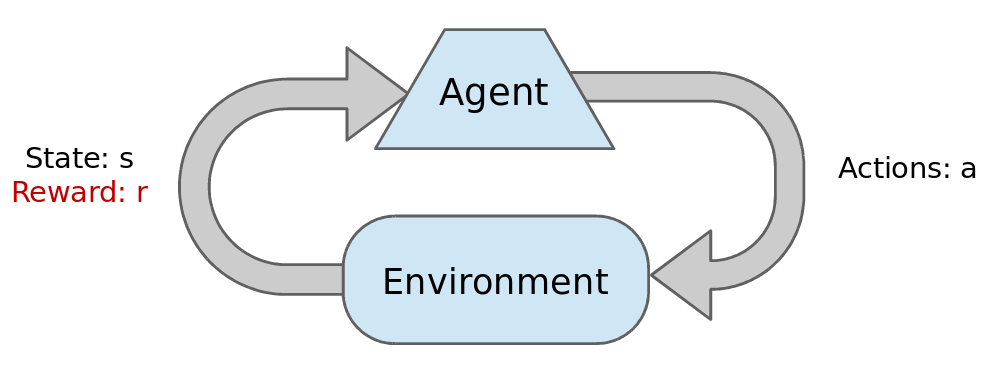
\includegraphics{img/learningagent.png}}
	\caption{Agent využívající strojové učení.}
	\label{img:learningagent}
\end{center}
\end{figure}

Metody strojového učení \cite{RLIntro}: se dělí dle \textbf{závislosti na modelu}
\begin{itemize}
\item (\textit{model-based}) metoda chce empiricky vytvořit model, který již lze řešit pomocí MDP - to se děje na základě průběžného výpočtu očekávaného užitku: 
\begin{enumerate}
\item spočítej všechny výsledky/vzorky $s^\prime$ pro každý pár $(s,a)$
\item spočítej odhad okamžitého užitku, tedy odhad přechodové funkce $\hat{T}(s,a,s^\prime)$
\item odhadni odměnovou funkci $\hat{R}(s,a,s^\prime)$ na základě objevených odměn stavů
\end{enumerate}
\item (\textit{model-free}) metoda model nepotřebuje, stačí posbírat vzorky, protože rozdělení pravděpodobnosti pro daný vzorek určuje jeho výskyt (není potřeba počítat očekávaný užitek). Dále se budeme zabývat těmito metodami.
\end{itemize}

Dalším dělicím kritériem je \textbf{řízení akcí}:
\begin{itemize}
\item \textit{pasivní} metody - je daná statická strategie $\pi(s)$, kterou se agent pevně řídí a získává z ní vzorky, ze kterých se učí hodnoty stavů $V(s^\prime)$ pro daný stav $s$.
\newline
Ukázka postupu metody přímého vyhodnocení (\textbf{direct evaluation} -ZDROJ-):
\begin{enumerate}
\item následuj $\pi$
\item pro každý navštívený stav vypočti sumu koeficientem $\gamma$ budoucích snížených hodnot
\item spočítej průměr sumy.
\end{enumerate}
Není potřeba $T$ ani $R$, avšak je zde přílišná abstrakce (plýtvání informací) a vyhodnocení stavů díky tomu má příliš velkou časovou náročnost.
\newline
Další možností je \textbf{Time-Difference value learning} \cite{RLIntro}, dále TD učení, které se místo vyhodnocování hodnoty Value iteration snaží vyhodnotit přímo nové strategie na základě hodnot (\textbf{Policy iteration}). Vyhodnocení probíhá \textit{po každé akci}, protože nelze zaručit, že se strategie bude vracet znovu do již vyhodnoceného stavu, aby opět přehodnotila svou hodnotu.
\begin{enumerate}
\item následuj $\pi$
\item aktualizuj $V(s)$ pokaždé, když narazíš na přechod pro vzorek $(s,a,s^\prime,r)$. \textbf{Aktualizace} (\textit{update}) spočívá v tom, že se vezme aktuální hodnota stavu a přičte se k ní o koeficient $\alpha$ zmenšený rozdíl mezi očekávaným stavem a reálným vzorkem. $\alpha$ reguluje fakt, že nové odměny budou mít větší váhu než staré.
-ROVNICE JSOU TUCNE, PREDELAT, PRECISLOVAT-  
\begin{displaymath}
\textrm{Vzorek $V(s)$:}\quad vzorek = R(s,\pi(s),s^\prime)+\gamma V^\pi(s^\prime)
\end{displaymath}
\begin{displaymath}
\textrm{Update $V(s)$:} \quad V^\pi(s) \leftarrow  V^\pi(s) + \alpha(vzorek - V^\pi(s))
\end{displaymath}
\end{enumerate}
TD učení je pasivní metoda, která je schopna získat ohodnocení hodnot $V$, avšak není schopna aktivně přeměnit hodnoty na novou strategii $\pi(s)$ dle rovnic MDP pro Policy iteration (viz obrázek \ref{img:policyeval} \cite{berkeley}):
\begin{displaymath}
\pi(s) = arg \max_a Q(s,a)
\end{displaymath}
\begin{displaymath}
Q(s,a) = \sum_{s^\prime}T(s,a,s^\prime) \left[R(s,a,s^\prime)+\gamma V(s^\prime) \right]
\end{displaymath}
Problém je opět chybějící přechodová a odměnová funkce ($T,R$), to řeší až aktivní metody strojového učení.

\begin{figure}[!htbp]
\begin{center}
	\scalebox{0.5}{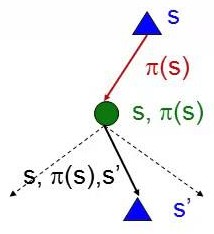
\includegraphics{img/policyeval.jpg}}
	\caption{Policy iteration metoda s potřebnými proměnnými.}
	\label{img:policyeval}
\end{center}
\end{figure}

\item \textit{aktivní} metody - je dána statická strategie $\pi(s)$, ale agent provádí vlastní akce a získává z nich vzorky, ze kterých se učí optimální strategie a hodnoty stavů $V(s^\prime)$. Mezi aktivní metody patří \textbf{Q-Learning}.
\end{itemize}

\subsection{Q-Learning}
Dosud se primárně vycházelo z $V$-hodnot, avšak Q-Learning staví na vyhodnocování posloupností akcí do nových stavů, tedy využití $Q$-hodnot. Jediné, co je tedy potřeba vědět je aktuální stav a jeho možné akce \cite{RLIntro}:
\begin{displaymath}
vzorek = \left [ R(s,a,s^\prime)+\gamma \max_{a^\prime}Q_{k}(s^\prime,a^\prime) \right]
\end{displaymath}
Následně se provede aktualizace (update) TD učení:
\begin{displaymath}
 Q(s,a) \leftarrow  Q(s,a) + \alpha(vzorek - Q(s,a))
\end{displaymath}
$\alpha$ nyní představuje rychlost učení (\textit{learning rate}).


\subsubsection{Q-Learning postup}
\begin{enumerate}
\item -POZOR NA PRAVY OKRAJ - ZAROVNANI-navštiv nový uzel a ze vzorku $(s,a,s^\prime,r)$ vypočti novou hodnotu jeho odhadu $Q_{k+1}(s,a)$ jako:
\newline
průměr očekávaných užitků akcí stavu $T\:*\:$ (okamžitá odměna $+$ nejlepší možná $Q$-hodnota následníka $Q_{k}(s,a)$), tedy:
\begin{displaymath}
Q_{k+1}(s,a) \leftarrow \sum_{s^\prime} T(s,a,s^\prime) \left[ R(s,a,s^\prime) + \gamma \max_{a^\prime} Q_k(s^\prime,a^\prime)\right]
\end{displaymath}
průměr $T$ a hodnoty odměn $R$ se postupně počítají na základě akcí (nejsou zpočátku známy), algoritmus se tedy blíží následující rovnici:

\begin{displaymath}
Q(s,a) \approx r + \gamma \max_{a^\prime}Q(s^\prime,a^\prime)
\end{displaymath}
$r$ je přímá odměna ze stavu

\item udělej update TD učení (průměr odhadu vůči vzorku)
\begin{displaymath}
 Q(s,a) \leftarrow  Q(s,a) + \alpha \left [ r + \gamma \max_{a^\prime} Q(s^\prime,a^\prime) \right]
\end{displaymath}
\end{enumerate}
Q-Learning konverguje k optimální strategii, i když následuje posloupnost neoptimálních akcí. Tento jev se nazývá \textit{off-policy learning} -ZDROJ-.
Jak ale agent vybírá, kterou akci provede, aby maximalizoval svůj užitek z tréninku? Je nutné zvolit dobrý poměr mezi zjišťováním terénu (\textit{exporation}) a využíváním již zjištěných dobrých strategií (\textit{exploitation}). Dobrý poměr lze řešit několika způsoby -ZDROJ-:
\begin{itemize}
\item zavedení koeficientu $\varepsilon-greedy$ pro výběr náhodných akcí. Výhodné je ovšem koeficient časem zmenšovat, aby nedocházelo k nelogičnostem akcí.
\item využití \textbf{explorační funkce}, která bere v potaz nejen budoucí užitek stavu $U$, ale i množství navštívění stavu $N$, tak aby se prozkoumaly stavy, jejichž špatná hodnota ještě není úplně jasná (málo výskytů). Funkce tedy snižuje důležitost opakujících se stavů a dává větší důraz na neprozkoumané stavy. Nakonec s tímto skončit, výsledný Q-Update potom vypadá:
\begin{displaymath}
Q(s,a) \leftarrow_\alpha R(s,a,s^\prime) + \gamma \max_{a^\prime} f(Q(s^\prime,a^\prime),N(s^\prime,a^\prime))\
\end{displaymath}
Q-Update se následně propaguje dál.
\end{itemize}
Novým pojmem pro metody posilovaného učení je \textbf{lítost} (\textit{regret}) jako míra toho, kolik mě stály všechny chyby během tréninku (rozdíl mezi očekávanými odměnami a optimálními odměnami). Je snaha tuto co nejvíce míru minimalizovat (optimálně se i učit optimální řešení daného problému).

\subsection{Approximační Q-Learning}
Zatímco základní Q-Learning pomohl zbavit se zbytečného přepočítávání hodnot, stále je potřeba si neustále udržovat tabulku všech $Q$-hodnot. Pro složitou úlohu jakou je Ms. Pacman je tato velká prostorová složitost stavového prostoru stále nevhodná. Z toho důvodu je potřeba \textbf{generalizovat}: naučit se Q-hodnoty malého množství tréninkových stavů a hodnoty generalizovat na podobných situacích. To je důležitá myšlenka metody aproximační Q-Learning a potažmo i strojového učení \cite{RLAprox}:
\newline
popsání stavu pomocí vektoru vlastností (\textit{properties}), vlastosti jsou funkce ze stavů do reálných čísel (např. 0,1), které zachycují důležité vlastnosti stavu. Následně lze tyto vlastnosti ohonodnotit \textbf{váhou} (\textit{weight}) a sesavit lineární rovnice \cite{RLAprox}:
\begin{displaymath}
V(s) = w_1f_1(s) + w_2f_2(s) + \dots + w_nf_n(s)
\end{displaymath}
\begin{displaymath}
Q(s,a) = w_1f_1(s,a) + w_2f_2(s,a) + \dots + w_nf_n(s,a)
\end{displaymath}
Nevýhoda takové generalizace je ale fakt, že je potřeba stanovit co nejlepší vektor vlastností tak, aby se hodnoty rozdílných stavů nepodobaly.
\subsubsection{Aproximační Q-Learning postup}

\begin{enumerate}

\item navštiv nový uzel a ze vzorku $(s,a,s^\prime,r)$ vypočti rozdíl odhadu Q-hodnoty vůči vzorku:
\begin{displaymath}
 rozdil = \left [ r + \gamma \max_{a^\prime}Q(s^\prime,a^\prime) \right]  - Q(s,a) 
\end{displaymath}
\item udělej update TD učení (průměr odhadu vůči vzorku)
\begin{displaymath}
 Q(s,a) \leftarrow  Q(s,a) + \alpha \left [ r + \gamma \max_{a^\prime}Q(s^\prime,a^\prime) \right]
\end{displaymath}
\item následně místo updatu jedné $Q$-hodnoty (základní Q-Learning), aproximuj $Q$-hodnoty pomocí změny váhy $w_i$ vůči vektoru vlastností:

\begin{displaymath}
w_i(s) \leftarrow w_i + \alpha \left [ r + \gamma \max_{a^\prime}Q(s^\prime,a^\prime) - Q(s,a) \right] f_i(s,a)
\end{displaymath}
kde:
\begin{itemize}
	\item $\left [ r + \gamma \max_{a^\prime}Q(s^\prime,a^\prime)\right] $ reprezentuje cíl (maximální), kterého se snaží daný stav dosáhnout (nejlepší odhad Q-hodnoty následujícího stavu)
	\item $\left [ Q(s,a)\right]$ vzorek aktuálního stavu
	\item $f_i(s,a)$ lineární funkce, jejíž rozdíl vzorků je aproximován\footnote{K aproximaci se používá obecná \textbf{Metoda nejmenších čtverců, tzv. lineární regrese}}, což napomáhá možnosti využití i nelineárních funkcí ve vektoru vlastností. Funkce reflektuje předpoklad odhadu Q-hodnoty následujícího stavu\newline
	Zjednodušeně řečeno např. u Ms. Pacman: Pokud Ms. Pacman narazí do ducha, zvětší se váha situace ohrožení Ms. Pacman duchem. Pokud se tedy stane nějaká pozitivní akce, pozitivní váha zvětší hodnoty vlastností ve vektoru vlastností a naopak.
\end{itemize}

\end{enumerate}

\chapter{Ms. Pacman}
\section{O hře a důvod jejího výběru}
\textit{Ms. Pacman} je arkádová hra z roku 1982, která vylepšuje původní koncept hry Pacman. Hra je obohacena o nový design hlavní postavy, mapy a především implementuje lepší umělou inteligenci nepřátel. Hlavní postavou ovládanou hráčem je nyní Ms. Pacman, nepřátelé zůstávají v podobě 4 barevných duchů. Cílem hry je dosáhnout co největšího skóre pojídáním kuliček, duchů (časově omezené; po snězení speciální větší kuličky tzv. power-upu), nebo ovoce.
Zvýšení obtížnosti oproti Pacmanovi spočívá především v \textbf{opuštění deterministického chování duchů}, čímž pádem nelze předpovídat jejich chování. Tento fakt spolu se složitostí hry jsou hlavními faktory proč se na hru zaměřit z hlediska strojového učení.
\section{Pravidla}
Pro účely této práce se bere v potaz zjednodušení původní hry na vizuální demo tak, aby byla dobře vidět účinnost jednotlivých algoritmů a nebyly příliš vysoké nároky na výpočetní výkon. Demo není rozděleno na levely, odehrává se na zvolené mapě a je založeno na umělé inteligenci obou stran (Ms. Pacman vs 2 duchové). Cíl Ms. Pacman je maximalizovat skóre na aktuální mapě, zatímco cíl nepřátel je její skóre minimalizovat. Stochastické chování nepřátel je simulováno tak, aby co nejvíce odpovídalo svému vzoru (zdrojové kódy hry nejsou veřejné, tudíž nelze simulovat chování duchů naprosto stejně jako v originálu). Duchové se snaží chytit a zabít Ms. Pacman. Pokud se jim to povede, hra končí (skóre -500 bodů). Skóre Ms. Pacman se navyšuje jezením jídla (skóre +10bodů za jednu kuličku), power-upů a následným jezením duchů (skóre +200 bodů za každého ducha) po omezený čas trvání power-upu. Bonusová ovoce se neberou v potaz. Skóre se snižuje po dobu chození Ms. Pacman po bludišti bez jezení ovoce/duchů. Mapy se též liší, jsou menší a obsahují pro umělou inteligenci Ms. Pacman problémová zákoutí, jako větší neohraničené plochy atp. Ms. Pacman a duchové mají stejnou rychlost. Tato zjednodušení slouží především ke snížení vypočetní náročnosti algorimů na běžně dostupný hardware.
\section{Klasifikace dema Ms. Pacman z hlediska Teorie her}
Ms. Pacman je hra, tzn. strategická interakce mezi 2 a více hráči, kteří chtějí dosáhnout optimálního výsledku ve hře.
Vizuální demo Ms. Pacman lze specifikovat podle několika kritérií:
\begin{itemize}
\item \textbf{dle informovanosti hráče o hře:} \textit{hra s neúplnou informací} (\textit{game with uncertainty}) - duchové mají stochastické chování
\item \textbf{dle počtu tahů:} \textit{hra strategická} – hráči provádějí souběžná rozhodnutí
\item \textbf{dle míry konkurence/typu výhry:} \textit{hra s nulovým součtem} (\textit{zero-sum game})  - jeden hráč maximalizuje svou výhru a druhý minimalizuje ztrátu (míra výhry jednoho značí míru prohry druhého hráče)
\item \textbf{dle počtu hráčů:} Ms. Pacman je maximizér a 2 duchové jsou minimizéři
\item \textbf{dle komunikace hráčů:} \textit{nekooperativní hra} – Ms. Pacman a duchové spolu nekomunikují a souběžně hrají proti sobě (striktně kompetitivní hra)
\item \textbf{dle zdrojů:} \textit{antagonistický konflikt} – Ms. Pacman a duchové sdílí jedno pevné maximální skóre
dle herního plánu: \textit{grid-world game} – vše probíhá diskrétně, po polích na mřížce v herním bludišti, jež mohou nabývat více stavů: prázdná cesta, zeď, prázdná cesta s hráčem, cesta s kuličkou, cesta s power-upem
\end{itemize}
\chapter{Návrh}
Tato kapitola se podílí na praktické části práce a to především návrhu \textbf{chování agentů}.
Po nastudování teorie je důležité jasně poupravit cíle práce: budou se porovnávat nejen metody Minimax a Alfa-Beta Řezy s učícím agentem, ale především také Expectimax, který bere v potaz stochastičnost akcí duchů. Tyto algoritmy se budou dále v textu označovat jako "základní algoritmy"

\section{Reflexivní agent a jeho ohodnocovací funkce}
Aby se měl učící agent s čím srovnat, bylo nutné navrhnout jednoduchého reflexivní agenta pracujícího s jednoduchou ohodnocovací funkcí. Reflexivní agent pouze vnímá aktuální stav hry (hloubka = 1) a jeho ohodnocovací funkce vyhodnocuje stav hry na základě informací o celém stavu hry. Agent se následně podívá na ohodnocení všech přípustných \textit{Akcí} (jít vlevo, vpravo, nahoru, dolů, zastavit se) a pseudonáhodně vybere mezi akcemi s nejlepším ohodnocením.  Jednoduchá \textbf{ohodnocovací funkce} agenta musí vzít v potaz především vzdálenosti jídla, duchů atp. Dále se bere v potaz stav ducha, zda ho dokáže Ms. Pacman dohonit tzn. kolik mu ještě zbývá kroků ve stavu vystrašenosti (Ms. Pacman snědla power-up) vůči jeho vzdálenosti od Ms.Pacman. Pro výpočet vzdáleností je použita tzv. manhattonovská metrika jako standard pro grid-world problematiku, tato vzdálenost je měřena jako suma rozdílu absolutních vzdáleností koordinát dvou bodů $\left|x1-x2\right|+\left|y1-y2\right|$.

\section{Minimax, AlfaBeta řezy}
Pro tyto algoritmy bylo nutné vzít v potaz větší počet minimalizujících nepřátel, kteří se v každém tahu dané hloubky střídají s maximalizující Ms. Pacman. Alfabeta i Minimax budou využívat stejnou nedokonalou vyhodnocovací funkci jako základní reflexivní agent, avšak navíc vyhodnotí stavy až do stanové hloubky/terminální uzlu a následně vrátí nejlepší možnou akci pro svého maximalizačního agenta Ms. Pacman (MinimaxAgent, AlphaBetaAgent).
\section{Expectimax a lepší ohodnocovací funkce}
Pro Expectimax agenta bude dále naimplementována vyhodnocovací funkce, která by měla dosáhnout lepších výsledků než funkce předchozích agentů. Popis, co je lepší, proč, jak by se to dále dalo vylepšit - například pomocí algoritmů pro prohledávání stavového prostoru.

\section{Value Iteration agent}
Tento agent je pasivní plánovací agent, nejdříve tedy provede veškeré své výpočty pomocí daného modelu světa a naplánuje si tak optimální posloupnost akcí, které se mají následně provést.
Z vypočetních a názorných důvodů, bude tento agent zobrazen výhradně formou již zmíněného \textbf{gridworld} problému (demonstrativní mřížka definovaná v souboru gridworld.py, na obr. XYZ)
Avšak určení nové hodnoty stavu $V$ poslouží i pro Q-Learningového agenta.

Velký vliv na jeho průběh mají především následující faktory:
koeficient odměny $\gamma$ - čím je koeficient menší, tím se vyhodnocení hodnot zpomaluje a důkladněji se tak prozkoumá více hodnot (výsledná posloupnost akcí může být například delší, ale optimálnější)
livingReward = ohodnocení pohybu z jednoho neterminálního stavu do druhého - čím je menší, až například záporná, tím rychleji se agent snaží najít terminální uzel a skončit tak hru/problém
noise = stochastičnost akce, tedy pravděpodobnost, že se daná akce provede - ovlivňuje, jak často agent riskuje

DÁL POPSAT, NEBO STACI JEN PSEUDOKOD REALIZACE???

\section{Q-Learning}
Hlavní náplní agenta je sestavit tabulku Q-hodnot každému páru (akce, stav) ve hře a následně z ních po stanoveném počtu iterací určit optimální strategii. Z názorných důvodů bude tento agent zobrazen formou \textbf{gridworld} problému a dále i ve hře Ms. Pacman.
STANOVENÍ ALFY,EPSILONU ATD...
STACI JEN REALIZACE ALGORITMU?
\section{Aproximační Q-Learning}
Důležitou částí návrhu řešení tohoto agenta je kvalitně definovat \textbf{vektor vlastností} (feature vector), který by měl korektně předpovídat $Q-hodnoty$ jednotlivých párů $(stav,akce)$:
\begin{itemize}
\item vzdálenost nejbližšího ducha a jeho stav
\item vzdálenost nejbližší kuličky jídla
\item vzdálenost nejbližšího power-upu
\item počet duchů
\end{itemize}
Následně se stanoví návrh aproximační funkce vektoru na základě váhy každé vlastnosti.

Poté bude především potřeba nalézt \textbf{optimální strategii}, která nebude pouze založena na již zmíněné metodě Aproximační Q-Learning:
\begin{enumerate}
\item aproximačně najdi model Q-hodnot
\item předpokládej pouze Q-hodnoty akcí z daného stavu
\item opakuj předchozí body dokud nebude dost vzorků, jinak pokračuj na další bod
\item poměňuj váhy vlastností a testuj optimálnost nové strategie
\end{enumerate}
Poměňování váh vlastností takto může \textbf{maximalizovat odměny} a dojít tak k lepší strategii, něž byla doposud použita.

\chapter{Realizace}
Tato kapitola popisuje praktickou část práce a především se zaměřuje na \textbf{implemetace různého chování agentů}.

\section{Zvolené prostředky}
Nejdříve bylo nutné si zvolit programovací jazyk, který by zvládl výpočetní náročnost problematiky vůči vykreslování grafického dema. Zpočátku byl zvolen jazyk Java díky její vysoké míře abstrakce vůči programátorskému myšlení. Nakonec však po sérii experimentování s jazykem se kvůli náročnosti samotné logiky hry vůči GUI a především kvůli efektivnímu zvládnutí rozgenerování všech možných stavů hry a dodržení matematických vzorců, jež byly stanoveny v předchozí teoretické kapitole, přešlo k hledání náhradního řešení. Tím se stalo hledání aplikace, nebo frameworku, jež řeší podobnou problematiku. Základem pro studii a experimentování s algoritmy nakonec posloužil pythonový framework od UC Berkeley \cite{pacmanProjects}, používaný v jejich výuce Úvod do umělé inteligence (kurz CS188) \cite{berkeley}. Hlavním důvodem zvolení frameworku bylo především zaměření práce na experimentování s algoritmy umělé inteligence, ne implemetace aplikace. Dalšími důvodem volby je použití jazyka \textit{Python 2.7.5}, který též umožňuje objektový přístup, je dobře čitelný a nenáročný - nejen díky těmto kladům se dají dobře pochopit vlastnosti a propojení jednotlivých objektů frameworku. Framework tedy primárně posloužil jako prostředek pro realizaci, srovnání a zobrazení výsledků jednotlivých algoritmů.
Pro účely této práce budou v následující sekcích popsány nejdůležitější části aplikace, detailní popis implementace frameworku lze najít v komentářích v kódu.

\section{Framework a reprezentace stavu hry}
Pro algoritmy je nejdůležitější částí frameworku objekt GameState reprezentující \textbf{stav hry}, který lze najít v souboru pacman.py (tento soubor a soubor game.py tvoří samotné jádro frameworku - definují základní chování agentů, možné akce, základní objekt stavového prostoru Grid apod.)
GameState dále pracuje s objekty PacmanRules a GhostRules, které zajišťují logiku pro svého agenta(agenty).
Tento základní objekt tedy obsahuje:
\begin{itemize}
\item pozice Ms.Pacman (index = 0) a duchů
\item pozice zbývajícího jídla v mřížce
\item pozice zbývajících power-upů v mřížce
\item pozice zdí v mřížce
\item počet duchů
\item možné akce, jež může daný agent provést z aktuálního stavu
\item schopnost provést akci a vytvořit tak svého následníka (objekt GameState)
\end{itemize}
Každý agent dědí ze základního objektu Agent povinnou metodu getAction (metoda, jež zavazuje agenta přijmout objekt GameSate a vrátit na něj reakci v podobě akce.) a proměnnou index definující index agenta (Ms. Pacman má tradičně index = 0).
Implementace vlastního chování konkrétního agenta je již definována v jeho konkrétním objektu (jako override). Např. AlphaBetaAgent přetěžuje metodu getAction jako algoritmus Alfa-Beta řezy atp.

\section{Reflexivní agent}
Pro srovnání s algoritmy byl implementován tento základní typ agenta. Největším problémem se stala jeho \textbf{ohodnocovací funkce}, neboť neustále narážela na problematické nesnadno vyřešitelné stavy stejného ohodnocení např. stejně vzdálené jídlo od agenta. Prakticky to pak dopadá, že agent doslova \textit{čeká} na ducha, aby se konečně mohl dostat ze zacykleného chování. Pro účely srovnání s následujícími agenty, však tento agent postačí.
-IMG- OBRÁZEK Z APLIKACE S VEKTORY VZDÁLENOSTÍ Na obrázku lze vidět problematické místo pro ohodnocovací funkci agenta, která je založena převším na vzdálenosti nejbližšího jídla vůči pozici agenta.

\section{Základní algorimy}
Jako ukázku lze uvést pseudokód algoritmu Expectimax, který je z hlediska porovnání s pokročilými metodami umělé inteligence nejzajímavější. Algoritmus musí mít přehled, která strana je na tahu na základě indexu agenta a také o kolikátou vrstvu střídání Ms. Pacman vs. (1-n) duchů se jedná - to zajišťuje proměnná depth.
\newline
-Pseudokód chování Agenta ExpectimaxAgent-:

def Expectimax(self, state, agentIndex, depth):

    nová vrstva
    if agentIndex == self.agentsNum:
        agentIndex = self.index
        depth += 1

    jedna se o terminalni uzel?
    if state.isWin() or state.isLose() or depth == self.depth:
        return self.evaluationFunction(state)

    Ms. Pacman
    if agentIndex == self.index:
        return maximize(state, agentIndex, depth)
    duchové
    else:
        return chanceMinimize(state, agentIndex, depth)

MAXIMALIZAČNÍ UZEL MS. PACMAN
def maximize(self, state, agentIndex, depth):

     tuple (action,value)
    value = ["", float("-inf")]
    for action in state.getLegalActions(agentIndex):
        tmp = self.Expectimax(state.generateSuccessor(agentIndex, action), agentIndex + 1, depth)
         getting value
        if type(tmp) is tuple:
            tmp = tmp[1]
        returning tuple with action
        if tmp > value[1]:
            value = (action, tmp)
    return value

UZEL NÁHODNOSTI
def chanceMinimize(self, state, agentIndex, depth):

     tuple (action,value)
    expectedValue = ["", 0.0]
    ghostActions = state.getLegalActions(agentIndex)

     ghost Actions probability
    probability = {}
    for action in ghostActions:
        probability[action] = 1.0 / float(len(ghostActions))

    for action in ghostActions:

        tmp = self.Expectimax(state.generateSuccessor(agentIndex, action), agentIndex + 1, depth)
         getting value
        if type(tmp) is tuple:
            tmp = tmp[1]

        expected action and value
        expectedValue[0] = action
        expectedValue[1] += tmp KRAT probability[action]
    return tuple(expectedValue)

\section{Framework a MDP problematika}
Hlavním objektem je ValueEstimationAgent (dědící od základní třídy Agent). Tento agent slouží především pro propojení prostředí problému (Ms. Pacman, gridworld) s $Q$-hodnotami párů (stav,akce), dále propojení stavu s jeho hodnotou ($V$) a nakonec propojení výsledných hodnot s nalezenou optimální strategiií.
Následující agenti od něj dále dědí následující základní metody:
\begin{itemize}
\item getQValue(state,action) - vrací Q-hodnotu páru (stav,akce)
\item getValue(state) - vrací hodnotu stavu (po vybrání nejlepší možné akce)
\item getPolicy(state) - vrací nejlepší možnou akci z daného stavu
\end{itemize}
\textbf{ValueIterationAgent} navíc potřebuje pro svoje chování model (přechodová funkce T, odměnová funkce R) a využívá pro to třídu MarkovDecisionProcess. MarkovDecisionProcess napojuje ve své metodě getTransitionStatesAndProbs(state, action) problematiku gridworldu na model, vrací tedy list párů $((s,a,s^\prime),T(s,a,s^\prime))$, tedy (následující možný stav z aktuálního stavu,jeho přechodová funkce = pravděpodobnost).
\newline
Abstraktní \textbf{ReinforcementAgent}, který je základním objektem pro agenty strojového učení, stará se o chování agenta během průbehu jednotlivých epizod, dále řeší vstupní argumenty a v případě Ms. Pacman o průběžný a finální výpis. Důležitými metodami jsou:
\begin{itemize}
\item observeTransition(state,action,nextState,deltaReward) -  voláno prostředím, které informuje agenta, že je získána nová hodnota přechodové funkce
\item update(state, action, nextState, reward) - updatování nových odhadů Q-hodnot
\end{itemize}
ReinforcementAgent staví na odhadu Q-Hodnot, protože neobsahuje model a je rodičem objektu řešící Q-Learning na gridworld problém \textbf{QLearningAgent}. Podobný agent, avšak s odlišnými vstupními parametry pro Ms. Pacman jsou \textbf{PacmanQAgent} a nakonec dále dědící \textbf{ApproximateQAgent}, který implementuje algoritmus Aproximační Q-learning a vyuřžívá u toho třídy FeatureExtractor pro implementaci vektoru vlastností pro Ms. Pacman.

\section{Value Iteration agent (ValueIterationAgent)}
%http://artint.info/html/ArtInt_227.html
-PSEUDOKÓD VALUE ITERATION???- ++ lepší popis v teorii!!! i s příkladem

\section{Q-Learning agenti (QLearningAgent,PacmanQAgent)}
Jak již bylo řešeno, tento agent si musí model odhadnout sám. Využívá k tomu především vhodný poměr prozkoumávání a uplatňování dosud zjištěného odhadu optimální akce z daného stavu (exporation/exploitation ratio). Tento poměr je dán parametrem $\epsilon-greedy$, který určuje náhodnost, zda se má provést optimální (pravděpodobnost $1-\epsilon$), či náhodná akce (pravděpodobnost $\epsilon$). Čím je $\epsilon-greedy$ větší, tím pravděpodobněji se agent chová dle své akuální optimální akce. Dalším důležitým faktorem je alfa($\alpha$), která ovlivňuje především rychlost učení. Čím je větší alfa, tím víc se dává důraz na nové vzorky.

\section{Aproximační Q-Learning agent (ApproximateQAgent)}

-PSEUDOKOD BETTERFEATUREXTRACTOR-

\chapter{Experimenty a srovnání agentů}
Agenty lze srovnat nejlépe podle dosaženého herního skóre.
\section{Srovnání z hlediska skóre}
\section{Srovnání z hlediska času}
\section{Výsledky}
učící křivka (x:skóre,y:počet tréninku)

\chapter{Závěr}
-PŘEPSAT-
Cílem toho semestrálního projektu bylo nastudovat problematiku metod hraní her ve vztahu k učícímu agentovi pro hru Ms. Pacman a navrhnout metodu řešení problému. Ms. Pacman. Nastudování teorie pomohlo především k definici a klasifikaci samotné hry jako problému umělé inteligence, a následném stanovení návrhu řešení problematiky metodou Aproximační Q-Learning. Tato metoda řeší stochastické chování duchů a pomůže výrazně eliminovat problém velké vypočetní náročnosti stavového prostoru Ms. Pacman. Jak si metoda s takto složitou problematikou poradí bude nejlépe vidět při srovnání její efektivity například s metodou Expectimax. Práce mě naučila především nebát se složitějších matematických vzorců a problémů a též určitý vhled do možností strojového učení.

